%%%%%%%%%%%%%%%%%%%%%%%%%%%%%%%%%%%%%%%%%%%%%%%%%%%%%%%%%%%%%%%%%%%%%%
%
% Autor: Gabriel Peres, João Carlos e Rodrigo Macedo
% Data:  04/10/2025
%
%%%%%%%%%%%%%%%%%%%%%%%%%%%%%%%%%%%%%%%%%%%%%%%%%%%%%%%%%%%%%%%%%%%%%%

\documentclass[12pt]{article}

\usepackage{sbc-template}
\usepackage{graphicx,url}
\usepackage[utf8]{inputenc}
\usepackage{hyphenat}

\sloppy

\title{Comparação de Algoritmos de Aprendizado Supervisionado em Problemas de Classificação}

\author{João Carlos dos Santos Correia, Gabriel Peres de Souza, Rodrigo Macedo Júnior}

\begin{document}

\maketitle

\begin{resumo}
Este artigo investiga a eficácia de algoritmos de aprendizado supervisionado para a detecção de eventos de grande público a partir de dados de tráfego. Utilizando o conjunto de dados "Dodgers Loop Sensor", foi realizado um estudo comparativo entre o desempenho da Regressão Logística, treinada com Gradiente Descendente Estocástico (SGD), e do k-Vizinhos Mais Próximos (k-NN). Os modelos foram avaliados por meio de validação cruzada com métricas como acurácia, precisão, revocação e AUC. Os resultados demonstram uma clara superioridade do k-NN, que alcançou uma acurácia de 97,37\% e AUC de 0.980, mostrando-se um classificador robusto e balanceado. Em contraste, a Regressão Logística apresentou utilidade prática limitada devido à sua precisão extremamente baixa.
\end{resumo}

\section{Introdução}
A análise de dados de sensores urbanos por meio de técnicas de aprendizado de máquina tem se tornado uma ferramenta poderosa para a compreensão de dinâmicas complexas, como o fluxo de tráfego e a ocorrência de eventos de grande porte. A capacidade de prever ou detectar tais eventos automaticamente pode otimizar o planejamento urbano, a gestão de tráfego e a alocação de recursos de segurança.

Este trabalho foca em um problema de classificação específico: a detecção de jogos de beisebol do time Dodgers, em Los Angeles, utilizando dados de um sensor de contagem de veículos. O desafio reside na natureza sutil do sinal, coletado em uma rampa de acesso estrategicamente posicionada para não tornar a detecção trivial, manifestando-se principalmente como um aumento no fluxo de saída ao final das partidas.
Conjunto
O objetivo deste artigo é comparar o desempenho de dois algoritmos de aprendizado supervisionado amplamente utilizados: a Regressão Logística, implementada com o otimizador Gradiente Descendente Estocástico (SGD), e o k-Vizinhos Mais Próximos (k-NN). Buscamos determinar qual modelo oferece a melhor capacidade de discriminação para esta tarefa, considerando um conjunto abrangente de métricas de avaliação.

Para alcançar este objetivo, o artigo está estruturado da seguinte forma: a Seção 2 detalha a metodologia, incluindo a descrição do conjunto de dados, os algoritmos e as métricas de avaliação. A Seção 3 apresenta e analisa os resultados comparativos dos modelos. Por fim, a Seção 4 oferece a conclusão do estudo, sintetizando os achados e destacando o modelo mais adequado para o problema proposto.

\section{Metodologia} \label{sec:metodologia}

\subsection{Conjunto de Dados}

O conjunto de dados empregado neste estudo é o "Dodgers Loop Sensor", proveniente do repositório UCI Machine Learning \cite{misc_dodgers_2010}. O objetivo central é a predição da ocorrência de jogos de beisebol do time Dodgers com base em anomalias no fluxo de tráfego.

Os dados consistem em medições de contagem de veículos, coletadas por um sensor de laço indutivo localizado em uma rampa de acesso para a rodovia 101 Norte em Los Angeles. As observações foram registradas continuamente ao longo de 25 semanas, com agregações a cada 5 minutos, totalizando 288 medições diárias. A localização do sensor foi estrategicamente posicionada próxima ao estádio, permitindo a captura de um sinal de tráfego sutil — mas não óbvio — que se manifesta principalmente ao final das partidas, quando os espectadores deixam o local.

\subsection{Algoritmos utilizados}

\subsubsection{Regressão Logística (treinada por Gradiente Descendente)}
A Regressão Logística modela diretamente a probabilidade da classe positiva por meio da função sigmoide
$\sigma(z) = \frac{1}{1 + e^{-z}}$, onde $z = \beta_0 + \sum_j \beta_j x_j$.
Os parâmetros $\beta$ são estimados por máxima verossimilhança, o que equivale a minimizar a perda logística
(entropia cruzada), conforme apresentado nos slides da disciplina \cite{naozuka_logistica_2025}.

\subsubsection{\texorpdfstring{$k$-Vizinhos Mais Próximos (k-NN)}{k-Vizinhos Mais Próximos (k-NN)}}
O k-NN é um método supervisionado baseado em instâncias: para um exemplo novo, calcula-se a distância para os exemplos de treino,
selecionam-se os $k$ vizinhos mais próximos e decide-se por votação da classe mais frequente (ou ponderada por distância).
É um algoritmo ``preguiçoso'' (sem fase explícita de treinamento), cuja qualidade depende da escolha de \emph{k} e da métrica de distância
\cite{naozuka_knn_2025}.

\subsection{Validação e seleção de hiperparâmetros}
Para estimar o desempenho fora da amostra e reduzir a variância da avaliação, utilizamos \textbf{validação cruzada k-fold estratificada} com $k=10$.

\subsection{Métricas de avaliação}
As métricas que reportamos derivam da \textbf{matriz de confusão} e foram trabalhadas em aula \cite{naozuka_metricas_2025}: Acurácia, Precisão, Revocação (Recall), F1-Score e a curva ROC com sua Área Sob a Curva (AUC).

\section{Resultados}

Nesta seção, os resultados da aplicação dos modelos de Regressão Logística (SGD) e k-NN são apresentados e analisados. A avaliação considera um limiar de decisão padrão de 0.5 para classificação.

\subsection{Desempenho Comparativo Geral}

A Figura \ref{fig:comparativo} apresenta uma comparação direta do desempenho dos dois modelos em todas as métricas de avaliação. Observa-se que o modelo k-NN obteve um desempenho superior em acurácia, precisão, f1-score e roc\_auc. Em contrapartida, o classificador SGD (Regressão Logística) demonstrou uma capacidade notavelmente maior de revocação.

\begin{figure}[h!]
    \centering
    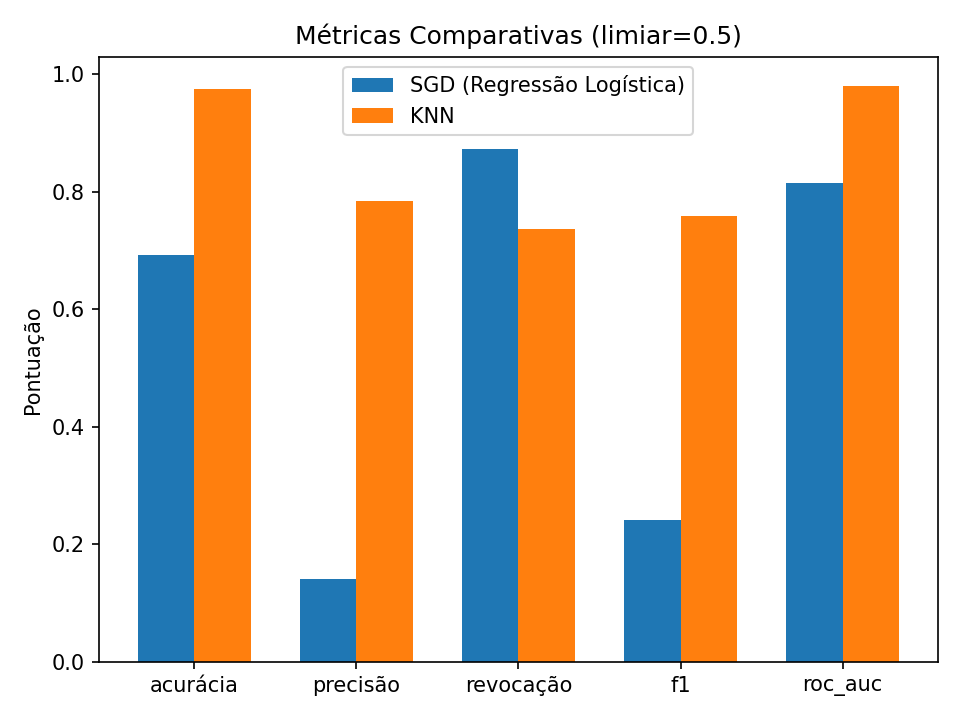
\includegraphics[width=0.8\textwidth]{image/metrics_comparison.png}
    \caption{Comparação de métricas entre os modelos SGD e k-NN com limiar de 0.5.}
    \label{fig:comparativo}
\end{figure}

\subsection{Análise do Modelo k-NN}
O modelo k-NN, após otimização de hiperparâmetros, utilizou $k=5$ vizinhos com a métrica de distância Euclidiana ($p=2$). Este modelo demonstrou ser altamente eficaz, atingindo uma acurácia global de \textbf{97,37\%}. Suas métricas de precisão (78,44\%) e revocação (73,55\%) são bem balanceadas, resultando em um f1-score de 75,92\%.

A matriz de confusão, apresentada na Tabela \ref{tab:knn_matrix}, detalha seu comportamento. O modelo classificou corretamente 46.986 instâncias como "não evento" e 2.089 como "evento", com um número relativamente baixo de erros (574 falsos positivos e 751 falsos negativos).

\begin{table}[h!]
    \centering
    \caption{Matriz de Confusão do Modelo k-NN.}
    \label{tab:knn_matrix}
    \begin{tabular}{cc|cc}
        & & \multicolumn{2}{c}{\textbf{Predito}} \\
        & & Não Evento & Evento \\ \hline
        \textbf{Real} & Não Evento & 46.986 & 574 \\
        & Evento & 751 & 2.089
    \end{tabular}
\end{table}

\subsection{Análise da Regressão Logística (SGD)}
O modelo de Regressão Logística, treinado com Gradiente Descendente Estocástico (SGD), apresentou um perfil de desempenho muito distinto. Embora tenha alcançado uma revocação altíssima de \textbf{87,18\%}, indicando que consegue identificar a maioria dos jogos que de fato ocorreram, sua precisão foi extremamente baixa, de apenas \textbf{14,06\%}.

Este desequilíbrio é evidenciado pela matriz de confusão na Tabela \ref{tab:sgd_matrix}. O modelo identificou corretamente 2.476 jogos, mas, para isso, gerou 15.129 falsos alarmes (falsos positivos). Esse comportamento torna o modelo pouco útil em um cenário prático, onde o custo de um alarme falso é relevante. O baixo f1-score (24,22\%) reflete essa falta de equilíbrio entre precisão e revocação.

\begin{table}[h!]
    \centering
    \caption{Matriz de Confusão do Modelo de Regressão Logística (SGD).}
    \label{tab:sgd_matrix}
    \begin{tabular}{cc|cc}
        & & \multicolumn{2}{c}{\textbf{Predito}} \\
        & & Não Evento & Evento \\ \hline
        \textbf{Real} & Não Evento & 32.431 & 15.129 \\
        & Evento & 364 & 2.476
    \end{tabular}
\end{table}

\subsection{Análise da Curva ROC}
A análise da Curva ROC (Figura \ref{fig:roc}) avalia a capacidade de discriminação dos modelos independentemente de um limiar de classificação específico. A Área Sob a Curva (AUC) confirma a superioridade do k-NN.

O modelo k-NN alcançou uma AUC de \textbf{0.980}, muito próxima do valor ideal de 1.0, indicando uma excelente capacidade de distinguir entre dias com e sem jogos. Em comparação, o modelo SGD obteve uma AUC de \textbf{0.814}, que, embora seja um resultado bom e muito superior a um classificador aleatório, é significativamente inferior ao do k-NN.

\begin{figure}[h!]
    \centering
    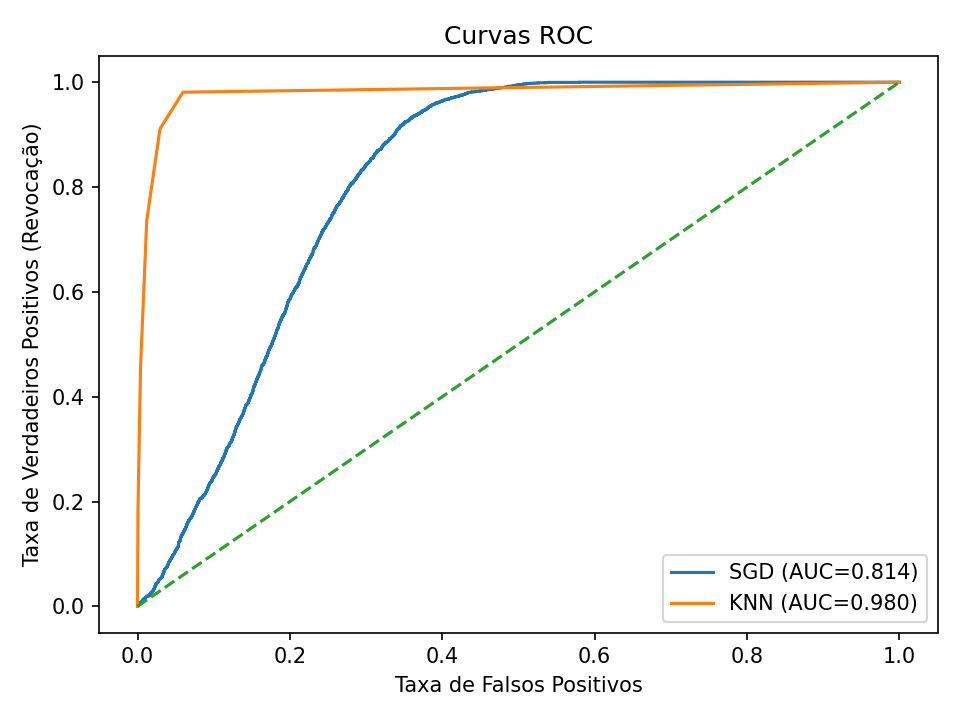
\includegraphics[width=0.8\textwidth]{image/roc_both.png}
    \caption{Curvas ROC e valores de AUC para os modelos k-NN e SGD.}
    \label{fig:roc}
\end{figure}


\section{Conclusão}

Os resultados demonstraram uma superioridade clara do modelo k-NN em quase todas as métricas de avaliação. Com uma acurácia de 97,37\% e uma AUC de 0.980, o k-NN provou ser não apenas preciso, mas também robusto na distinção entre as classes. Seu equilíbrio entre precisão (78,44\%) e revocação (73,55\%) o torna um classificador confiável e prático para este problema.

Por outro lado, a Regressão Logística, embora tenha alcançado uma alta revocação (87,18\%), o fez ao custo de uma precisão drasticamente baixa (14,06\%), gerando um número excessivo de falsos positivos. Este comportamento indica que o modelo tende a classificar muitas instâncias como positivas, o que, dependendo da aplicação, pode ser indesejável.

Conclui-se que, para este conjunto de dados e problema de classificação, a capacidade do k-NN de capturar padrões locais complexos, sem assumir uma fronteira de decisão linear, foi fundamental para seu desempenho superior. A Regressão Logística, apesar de sua simplicidade e interpretabilidade, não foi capaz de modelar a relação entre o tráfego e a ocorrência dos eventos com a mesma eficácia.

\bibliographystyle{sbc}
\bibliography{referencias,sbc-template}

\end{document}